\documentclass[journal]{./IEEE/IEEEtran}
\usepackage{cite,graphicx}
\newcommand{\SPTITLE}{An Educational Tool for Basic Sign Language Gestures Detection using React.JS and Tensorflow.JS}
\newcommand{\ADVISEE}{Mark Oliver D. Fojas}
\newcommand{\ADVISER}{Joseph Anthony Hermocilla}

\newcommand{\BSCS}{Bachelor of Science in Computer Science}
\newcommand{\ICS}{Institute of Computer Science}
\newcommand{\UPLB}{University of the Philippines Los Ba\~{n}os}
\newcommand{\REMARK}{\thanks{Presented to the Faculty of the \ICS, \UPLB\
                             in partial fulfillment of the requirements
                             for the Degree of \BSCS}}
        
\markboth{CMSC 191 Special Problem, \ICS}{}
\title{\SPTITLE}
\author{\ADVISEE~and~\ADVISER%
\REMARK
}
\pubid{\copyright~2022~ICS \UPLB}

%%%%%%%%%%%%%%%%%%%%%%%%%%%%%%%%%%%%%%%%%%%%%%%%%%%%%%%%%%%%%%%%%%%%%%%%%%

\begin{document}

% TITLE
\maketitle

% ABSTRACT
\begin{abstract}
The abstract should be \textit{informational}. Typically a single paragraph
of about fifty to two hundred workds, the abstract allows your readers to judge
whether or not the article is of relevance to them. It should therefore be
a concise summary of the aims, scope, and conclusions of your work. There
is no space for unnecessary texts; an abstract should be kept to as few words
as possible while remaining reasonably informative. Irrelevancies, such as
minor details or a \textit{description} of the structure of the paper, are 
inappropriate, as are acronyms, abbreviations, and mathematics. Sentences such
as ``we review relevant literature" should be omitted.\cite{Zobel97}
\end{abstract}

% INDEX TERMS
\begin{keywords}
ASL, FSL, PWD, TFJS, key, words, separated, by, comma
\end{keywords}

% INTRODUCTION
\section{Introduction}
To be effective, the introduction should answer the questions ``Why and What For (Four)?" Expanded, these questions are:\cite{Papadakis83}

\subsection{Why is the topic of interest?}
Start paragraph here...

\subsection{What is the background on the previous solutions, if any?}
Start of first paragraph. The quick brown fox jumps over the lazy dog. The quick
brown fox jumps over the lazy dog. The quick brown fox jumps over the lazy dog. The
quick brown fox jumps over the lazy dog.

Start of second paragraph. The quick brown fox jumps over the lazy dog. The quick
brown fox jumps over the lazy dog. The quick brown fox jumps over the lazy dog. The
quick brown fox jumps over the lazy dog.

\subsection{What is the background on potential solutions}

\subsection{What was attempted in the present effor (research project)?}

\subsection{What will be presented in this paper?}
Subsection text here.
\par
Sign Language is a form of visual communication that incorporates hand signs, gestures, facial expressions, and body language to convey a message. It provides natural means of communication between persons with disabilities and the elderly alike. [13] According to (Davis et al. 1997; Kuhl and Williams 1992), 80–90\% of youngsters have a persistent, substantial hearing impairment present since the neonatal period. The key developmental issue for the majority of newborns with hearing loss is language development and the accompanying domains that depend on timely language acquisition, for example, cognition and socioemotional development. Problems arise as the majority of families with deaf children do not know sign language, creating a communication mismatch. [1] Attempts to resolve the said mismatch of often done using technology such as hearing aids or cochlear implants while not taking advantage of visual learning like sign language.
\par
According to Aleem, Yousuf, Mehmood, Suleman, Sameer, Razi, Rehman and Israr, 2005, sign language is not universal. Misconceptions about sign language are that it is easy to learn [2], and that early exposure to natural sign languages hinders the development of spoken language.[22] Sign Language varies from different country and an example of sign language is ASL or American Sign Language. While the basic signs of this language are commonly known and iconic like the signs for sleep and drink, ASL is a complex language that requires constant practice and exposure. [2] FSL, also known as Filipino Sign Language, is another sign language that is used in the Philippines. FSL has a linguistic structural hierarchy based on a manual signal reinforced by extra linguistic information from non-manual signals of the face and body. Filipino Sign Language provides 26 signs for the alphabet and has various other gestures to denote phrases. Learning ASL, and other sign language should be approached respectfully and with the understanding that proficiency only comes after a long period of practice.
\par
With the popularity of computing devices, the necessity of practical and user friendly computer interfaces arise. Systems using vision-based interaction are becoming increasingly common, as well as gesture recognition systems. Previous efforts to create systems of gesture recognition incorporating sign language can be seen on the works of [26],  [27], and [28]. 
\par
In this study, FSL will be substituted in the place of ASL. A system using Tensorflow, HandPose, and React.JS will be created to recognize signs from FSL. It will utilize Google’s Tensorflow, which is a free and open-source library for machine learning and artificial intelligence. React.JS will be used to create the Application to create the system for the recognition of signs. This would help deaf-mute or hearing-impaired Filipinos to have an access to materials for learning or testing how correct their knowledge of FSL.
\par
The main challenge in this study is to optimize the recognition system and the training of the machine learning to be as precise as possible. Since this is a vision-based recognition system, it is subjected to constraints such as preciseness, lightning condition, background noises, and hardware speed.


%RELATED WORK
\section{Related Work}
\par
There have been previous attempts to create a system that recognizes sign language. There are some works done in different sign languages, and different deep learning, machine learning, or using convolutional neural networks.
\par
S. Shivashankara and S. Srinath [26], presented various algorithm and techniques in sign language recognition process. They were able to discuss 27 techniques:  Feed forward artificial neural network (ANN), Backpropagation, Canny Edge Detectors, Speed up Robust Features(SURF), Madaline, AdaBoost Classifiers, Haar Classifiers, K-Curvature, Convex Hull, Morphological operations, Seeded Region Growing (SRG) Algorithm, Principal Component Analysis (PCA), Hidden Markov Model (HMM),  Point Distribution Model (PDM), Kalman Filtering,  Fuzzy Decision Trees, Discrete Cosine Transform (DCT), K-Nearest Neighbors Algorithm (K-NN), Support Vector Machines (SVMs), Naive Bayes Classifiers, Probabilistic Neural Network (PNN), Cartesian Genetic Programming (CGP), Self-Organizing Map (SOM), and Finite-State Machines (FSM). Each of the algorithms processes are explained as well as their results and remarks. 
\par
Köpüklü, et al [27] developed a system that recognizes gestures and classifies them in real-time using convolutional neural networks (CNN). They used the EgoGesture Dataset [N], and NVIDIA Dynamic Hand Gesture Dataset[] as data for training, and C3D [N] and ResNeXt-101[N] where used for their CNN. ResNeXt101 architecture are used to achieve the offline classification accuracies of 94.03\% and 83.82\% on depth modality.
\par
Eyob Gebretinsae [28] also designed and developed a system for video-based finger spelling recognition for Ethopian Sign Language (ESL) using center of mass and finite state automata from a video. Preprocessing, image segmentation, and post processing are done before trying to understand signs from key frames in the video. Images are processed using signed hand segmentation to define the signed hand from the input. Preprocessing and post processing are done to accurately recognize the signs. The center of mass is defined for each signed hand, and is used to detect the motion and recognize vowels from ESL, finite state automata are used to recognize vowels. They claim to have an overall system recognition performance is 90.75\% which means that 216 out of a total of 238 finger spellings are recognized. 
\par
M. Jaberese, et al [29], developed a real-time sign-to-speech convolutional neural network-based Filipino Sign Language Hand Gesture Recognition system. They used 237 video clips of 20 different gestures. Data cleaning and augmentation using pre-processing techniques were used in the dataset to efficiently train the CNN used. An Inflated 3D CNN was used to train the Filipino Sign Language recognition system. Using the Rapid Application development model, they claim that the application created was deemed effective and efficient.


% MATERIALS AND METHODS
\section{Materials and Methods}
\subsection{Data Collection and Image Labeling}
\par
A set of N images for each of the 27 FSL Alphabet  will be collected and used as a dataset for training the neural network. Each image will be named according to the sign related to the image and would be added a unique identifier using python’s UUID library. LabelImg (Label Image), an open-source tool for graphically labeling images will be used to annotate and label the signed hands in each image. Ten percent of each set of images will be moved to the testing directory and the remaining 90\% will be moved to the training directory as well as the generated XML files. This labeled dataset will be used for training the said neural network.

\subsection{Training Of Neural Network}
\par
A \'label map\' would be created for each sign that would be recognized in the system. Google\'s Tensorflow would be used to create a python script to convert the XML annotations from the labeled dataset to the TensorFlow records for training and testing. This step is critical to ensure that the data will be in the right format before training and testing. SSD Mobilenet is the model that will be used from the Tensorflow Model Zoo as it is optimized for speed. The pipeline configuration will be set up for transfer learning before starting to train the model. The model will then be trained using the Tensorflow training record created with minimum training steps of N.
The trained model will then be converted to TFJS model using tensorflowjs converter.  Cloud Object Storage in IBM cloud will be used to host the TFJS model. The model as well as the created bin files will then be uploaded to the IBM Cloud. Cross-Origin Resource Sharing (CORS) will be enabled to allow access of the models and bin files from the system that will be created. IBM Cloud CLI will be used for setting up CORS configuration. 

\subsection{Computer Vision Application}
\par
A computer vision application will be developed using React. A neural network will be created that will use the hosted model. The application will get input from the connected webcam, to make detection, the extracted frame will then be transformed into pixel values, resized, cast into Int\-32, and set up the data into the array our model expects the data to be. The neural network will be used to make detections from the pre-processed image. A drawing function will be defined that will use the data that we will get from the detection results. This will draw the bounding box for the detected sign, the accuracy of the detection, and display the meaning of the sign detected. 

% RESULTS AND DISCUSSION
\section{Results and Discussion}
Sample Sentence

% CONCLUSION AND FUTURE WORK
\section{Conclusion and Future Work}
Sample Sentence

% APPENDICES
\appendices

\section{Proof of the First Zonklar Equation}
Appendix one text goes here...

\section{}
Appendix two (without title) text goes here...

% ACKNOWLEDGMENT
\section*{Acknowledgment}
Many thanks to...

% BIBLIOGRAPHY
\bibliographystyle{./IEEE/IEEEtran}
% \bibliography{./fojas-cs190-ieee}
% \nocite{*}

% BIOGRAPHY
\begin{biography}[{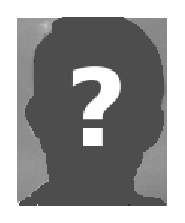
\includegraphics{./yourPicture.eps}}]{\ADVISEE}
Biography text here...
\end{biography}


\end{document}
 
